\chapter{Results}

This section provides the main results of the investigation. First, the results reproduced from the original paper \cite{notarmuzi2021percolation} are presented. Then, the results of
the analysis with $n=2$ are shown. Finally, we have studied the behaviour of an inhibitory and excitatory neuron coupled.

\section{Results from the original paper}

The first result is the percolation phase diagram is shown in Figure \ref{f:phase_diagram_article}. It displays the percolation strength $P_{\infty}$ versus the resolution parameter $\Delta$.

\begin{figure}[H]
    \centering
    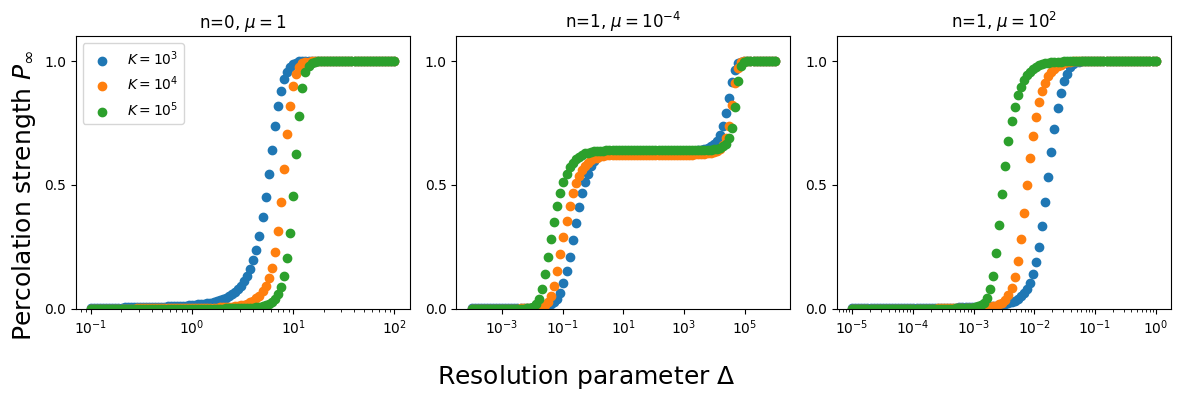
\includegraphics[width=0.95\textwidth]{phase_article_R=1000.png}
    \caption{Percolation phase diagrams for different event number $K$ taking average values of $R=1000$ realizations.}
    \label{f:phase_diagram_article}
\end{figure}

The first plot configuration is a Markovian ($n=0$) Poisson process with rate $\mu$. This is the simplest case, where the inter-event time $x=t_i-t_{i-1}$ follows an exponential 
distribution $P(x_i)=\mu e^{\mu x_i}$. The other two plots are non-Markovian Hawkes processes for $\mu \ll 1$ and $\mu\gg 1$. In one hand, a double transition is observed when 
$\mu = 10^{-4}$, in the other hand, a single transition occurs when $\mu = 10^2$. 

Once we have the phase diagram, we can study the avalanches' statistics at different regions of it. Given a resolution parameter $\Delta$, we can spot clusters or avalanches of activity.
A cluster starts when a neuron fires and ends if the neuron does not fire for a time greater than $\Delta$. We define the size of a cluster as the number of spikes it contains and the duration
as the time between the first and last spike. We have studied the avalanches for $K=10^5$ events and $R=1000$ realizations to obtain the average values since the process is highly not 
stationary. We will study the size and duration of the avalanches for the three different regions of the phase diagram for $\mu=10^{-4}$ and the two regions of the phase diagram for $\mu=10^2$.



\section{Results for n=2}

In the article, the authors have studied a process which is critical itself because $n=1$. We have studied the case $n=2$ to see if the process is still critical. Simillary to the 
previous section, we obtaine the phase diagram to observe the resolution parameter of the phase transition and after that we have studied the avalanches' statistics for the different
regions.

\begin{figure}[H]
    \centering
    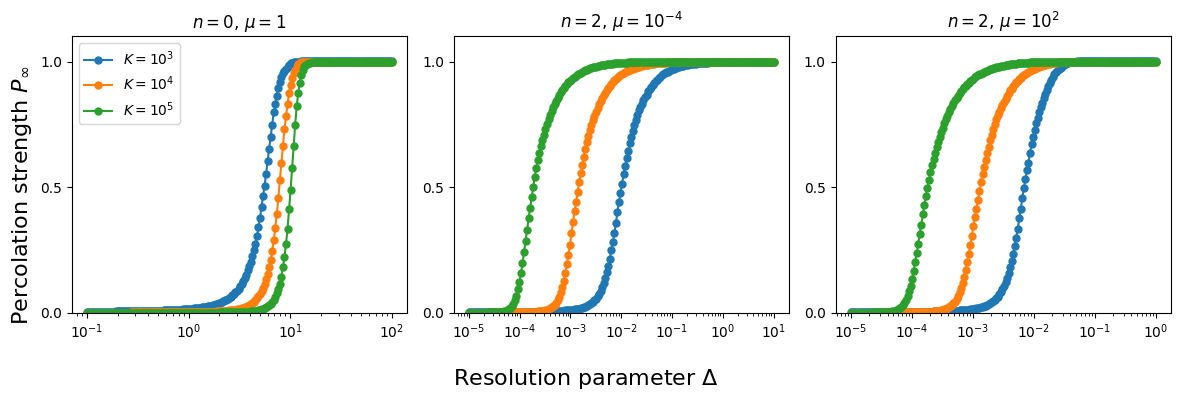
\includegraphics[width=0.95\textwidth]{phase_R=1000_n=2.png}
    \caption{Percolation phase diagrams for a Hawkes process with $n=2$.}
    \label{f:phase_diagram_n=2}
\end{figure}

\begin{figure}[H]
    \centering
    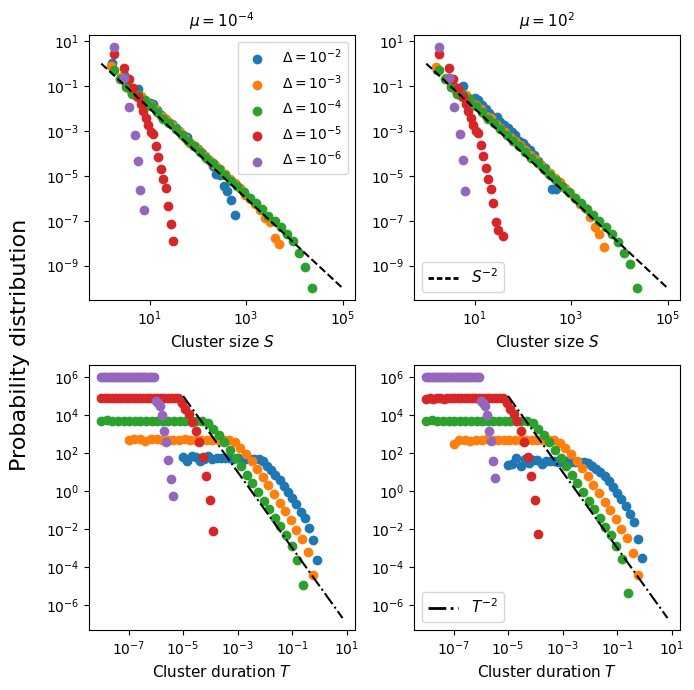
\includegraphics[width=0.95\textwidth]{cutoff_data_dots_n=2.png}
    \caption{Avalanches' statistics for a Hawkes process with $n=2$.}
    \label{f:avalanches_n=2}
\end{figure}